\section{Deployment View}

\begin{figure}[H]
	\centering
	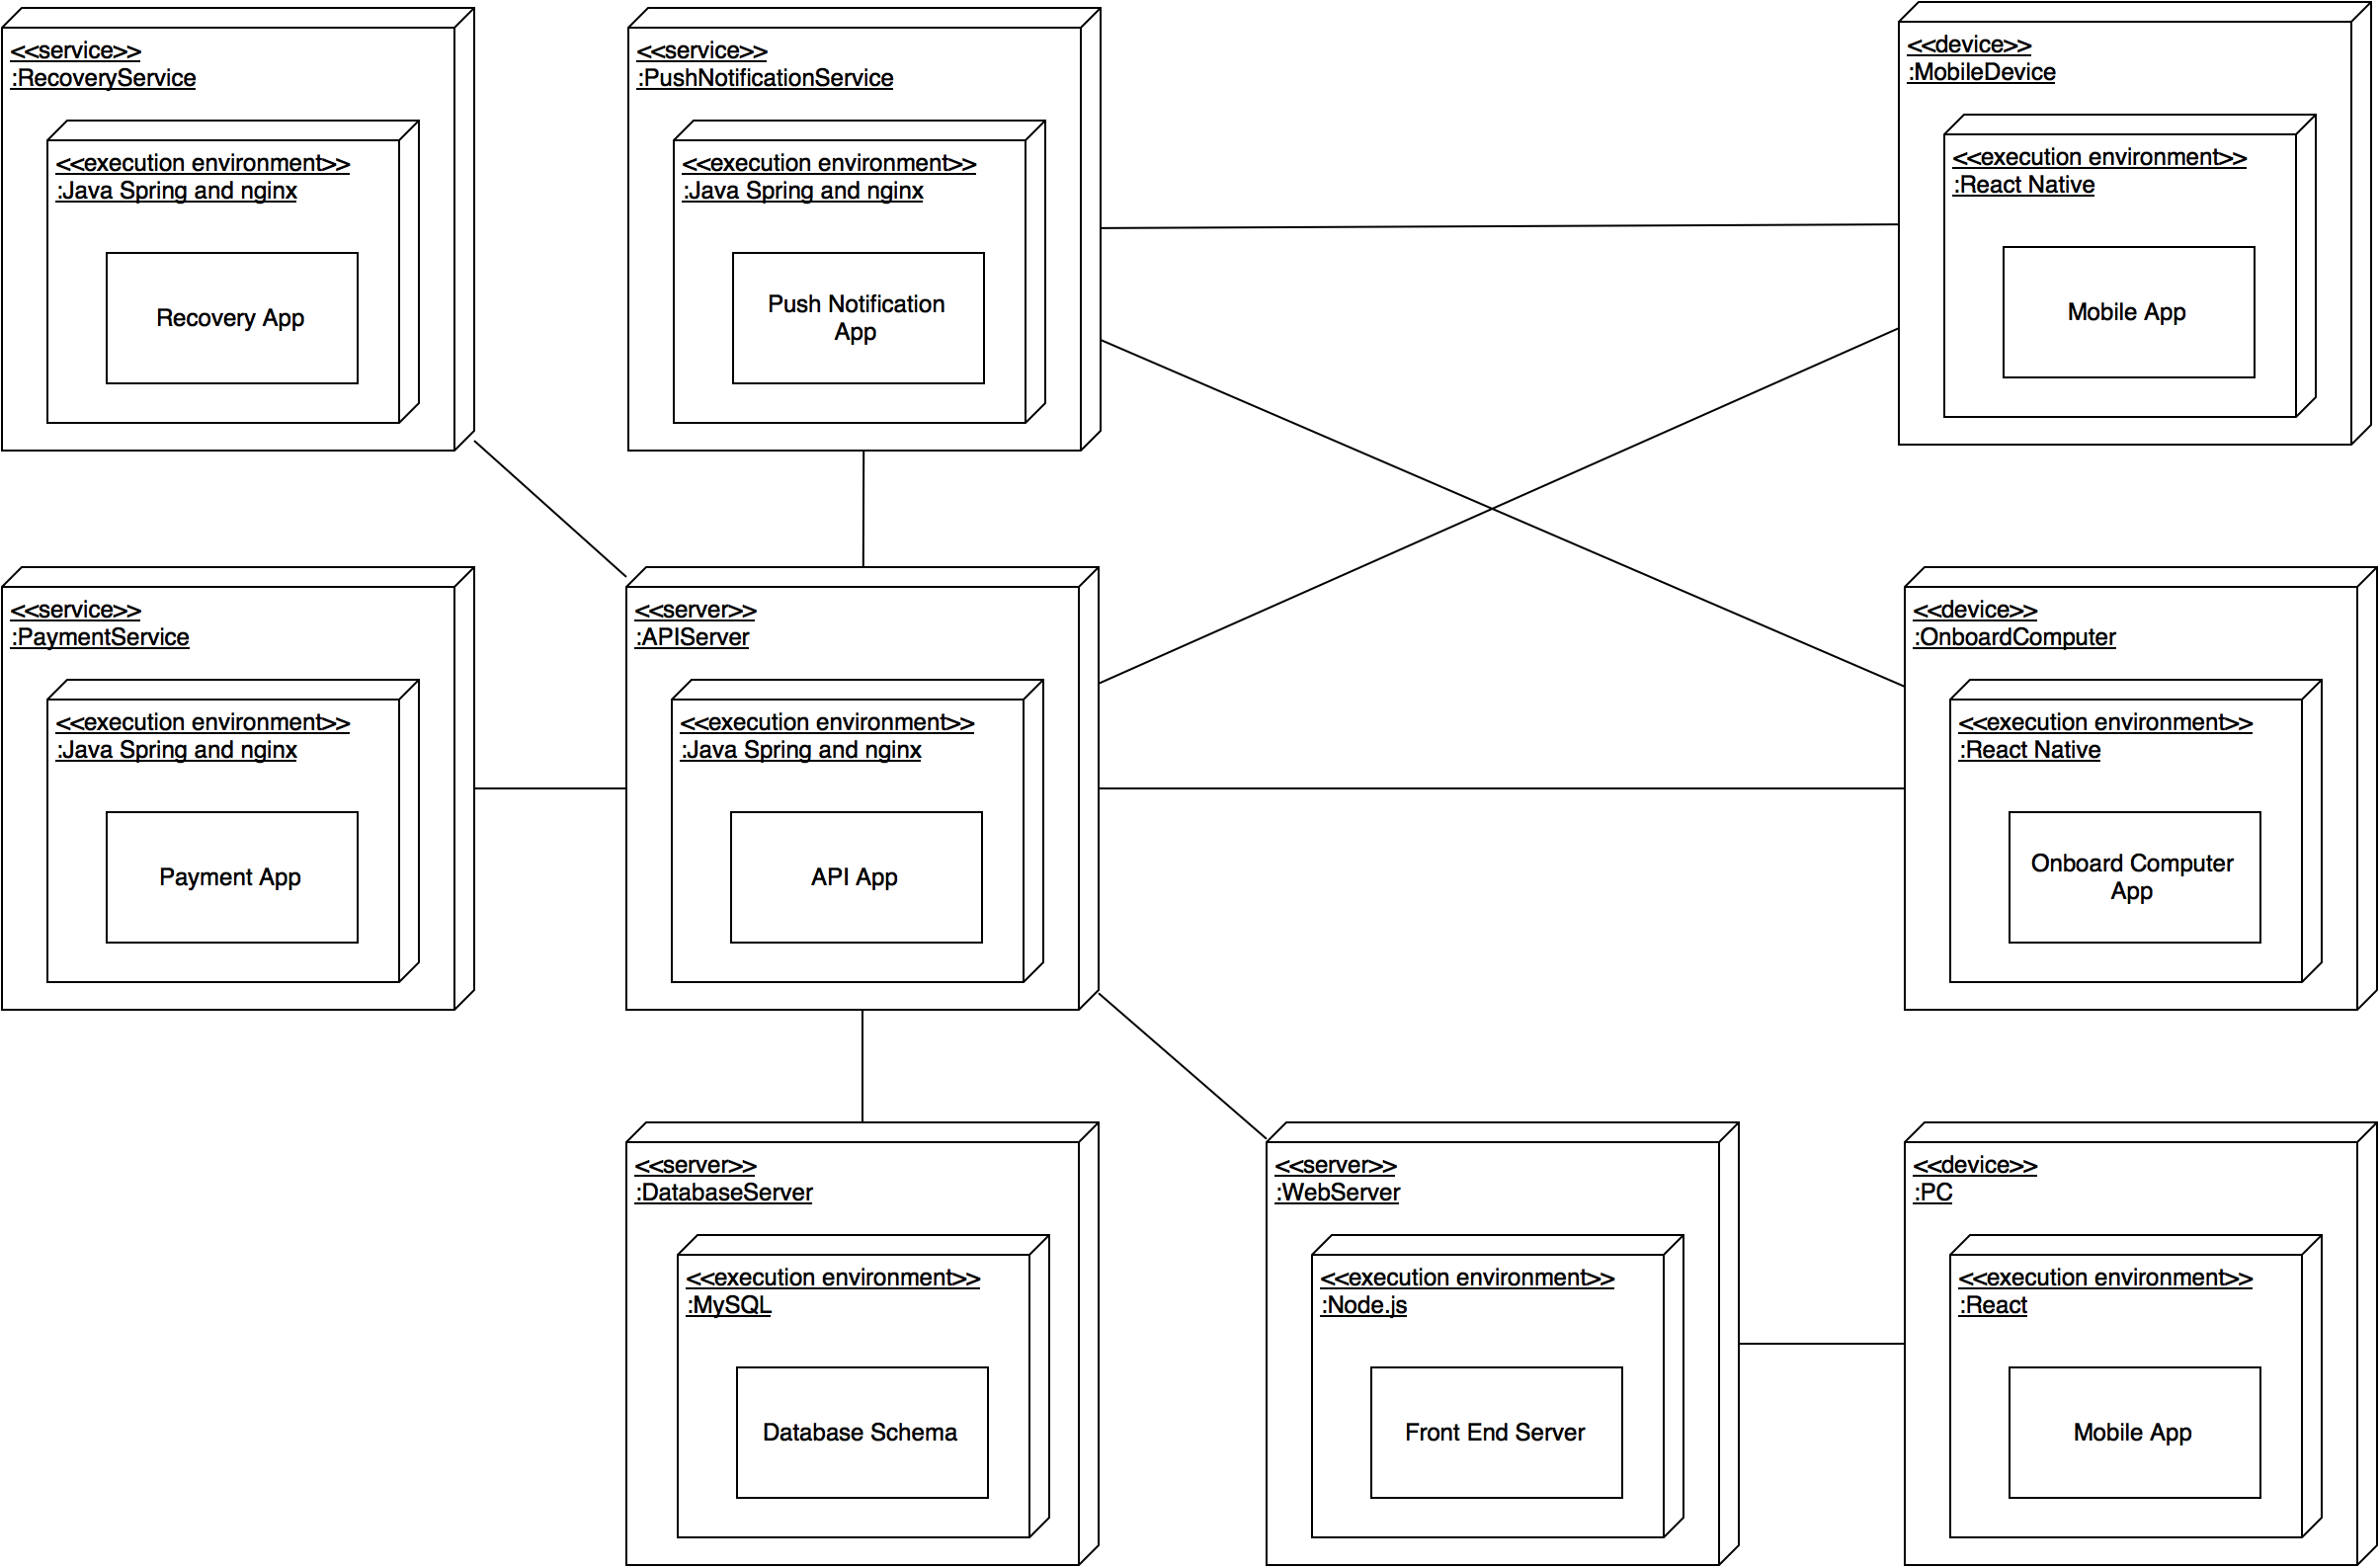
\includegraphics[width=1.4\textwidth, angle=90]{deployment-diagram}
	\caption[Deployment Diagram]{The picture above provides an overall description of the system architecture components and their interactions.}
	\label{fig:deployment}
\end{figure}

From an high level point of view, the deployment view shows the three tiers of the system architecture: client (MobileDevice, PC, OnboardComputer), application (APIServer, WebServer and Services) and data (DatabaseServer). There are some new aspects that have been introduced in this diagram and which have not been mentioned previously. For this reason, further details about them will be given below.

The WebServer is a useful component with respect to the desktop web application. The WebServer contains all the static content of the web pages. This pattern allows the clients to render only the dynamic content of the web pages, such as dynamic data arriving from the APIServer and animations.

The Services, e.g. payment, recovery and notification, provide the system with APIs that can be used to invoke the functions required. For example, in order to execute a payment, the system will call a specific end-point of the PaymentService with the necessary information about the payment requested.

Below, the list of frameworks mentioned in the deployment diagram is provided.

\paragraph{Back End}
\begin{itemize}
	\item Java Spring \cite{spring}
	\item nginx \cite{nginx}
	\item Node.js \cite{nodejs}
	\item MySQL {\cite{mysql}}
\end{itemize}

\paragraph{Front End}
\begin{itemize}
	\item React \cite{react}
	\item React Native \cite{react-native}
\end{itemize}
